% Options for packages loaded elsewhere
\PassOptionsToPackage{unicode}{hyperref}
\PassOptionsToPackage{hyphens}{url}
%
\documentclass[
  10pt,
  ignorenonframetext,
  compress]{beamer}
\usepackage{pgfpages}
\setbeamertemplate{caption}[numbered]
\setbeamertemplate{caption label separator}{: }
\setbeamercolor{caption name}{fg=normal text.fg}
\beamertemplatenavigationsymbolsempty
% Prevent slide breaks in the middle of a paragraph
\widowpenalties 1 10000
\raggedbottom
\setbeamertemplate{part page}{
  \centering
  \begin{beamercolorbox}[sep=16pt,center]{part title}
    \usebeamerfont{part title}\insertpart\par
  \end{beamercolorbox}
}
\setbeamertemplate{section page}{
  \centering
  \begin{beamercolorbox}[sep=12pt,center]{part title}
    \usebeamerfont{section title}\insertsection\par
  \end{beamercolorbox}
}
\setbeamertemplate{subsection page}{
  \centering
  \begin{beamercolorbox}[sep=8pt,center]{part title}
    \usebeamerfont{subsection title}\insertsubsection\par
  \end{beamercolorbox}
}
\AtBeginPart{
  \frame{\partpage}
}
\AtBeginSection{
  \ifbibliography
  \else
    \frame{\sectionpage}
  \fi
}
\AtBeginSubsection{
  \frame{\subsectionpage}
}
\usepackage{lmodern}
\usepackage{amssymb,amsmath}
\usepackage{ifxetex,ifluatex}
\ifnum 0\ifxetex 1\fi\ifluatex 1\fi=0 % if pdftex
  \usepackage[T1]{fontenc}
  \usepackage[utf8]{inputenc}
  \usepackage{textcomp} % provide euro and other symbols
\else % if luatex or xetex
  \usepackage{unicode-math}
  \defaultfontfeatures{Scale=MatchLowercase}
  \defaultfontfeatures[\rmfamily]{Ligatures=TeX,Scale=1}
\fi
\usetheme[]{boxes}
\usefonttheme{structurebold}
% Use upquote if available, for straight quotes in verbatim environments
\IfFileExists{upquote.sty}{\usepackage{upquote}}{}
\IfFileExists{microtype.sty}{% use microtype if available
  \usepackage[]{microtype}
  \UseMicrotypeSet[protrusion]{basicmath} % disable protrusion for tt fonts
}{}
\makeatletter
\@ifundefined{KOMAClassName}{% if non-KOMA class
  \IfFileExists{parskip.sty}{%
    \usepackage{parskip}
  }{% else
    \setlength{\parindent}{0pt}
    \setlength{\parskip}{6pt plus 2pt minus 1pt}}
}{% if KOMA class
  \KOMAoptions{parskip=half}}
\makeatother
\usepackage{xcolor}
\IfFileExists{xurl.sty}{\usepackage{xurl}}{} % add URL line breaks if available
\IfFileExists{bookmark.sty}{\usepackage{bookmark}}{\usepackage{hyperref}}
\hypersetup{
  pdftitle={Changes in extremes},
  hidelinks,
  pdfcreator={LaTeX via pandoc}}
\urlstyle{same} % disable monospaced font for URLs
\newif\ifbibliography
\usepackage{longtable,booktabs}
\usepackage{caption}
% Make caption package work with longtable
\makeatletter
\def\fnum@table{\tablename~\thetable}
\makeatother
\usepackage{graphicx,grffile}
\makeatletter
\def\maxwidth{\ifdim\Gin@nat@width>\linewidth\linewidth\else\Gin@nat@width\fi}
\def\maxheight{\ifdim\Gin@nat@height>\textheight\textheight\else\Gin@nat@height\fi}
\makeatother
% Scale images if necessary, so that they will not overflow the page
% margins by default, and it is still possible to overwrite the defaults
% using explicit options in \includegraphics[width, height, ...]{}
\setkeys{Gin}{width=\maxwidth,height=\maxheight,keepaspectratio}
% Set default figure placement to htbp
\makeatletter
\def\fps@figure{htbp}
\makeatother
\setlength{\emergencystretch}{3em} % prevent overfull lines
\providecommand{\tightlist}{%
  \setlength{\itemsep}{0pt}\setlength{\parskip}{0pt}}
\setcounter{secnumdepth}{-\maxdimen} % remove section numbering
\usepackage{amsmath, amssymb}

\definecolor{univered}{rgb}{0.75,0.01,0.3}\definecolor{darkred}{RGB}{154,2,0}
\beamertemplatenavigationsymbolsempty\setbeamercovered{invisible}\setbeamercolor{item projected}{bg=univered}\hypersetup{colorlinks,citecolor=univered,filecolor=univered,linkcolor=univered,urlcolor=univered}\setbeamertemplate{footline}{\leavevmode\begin{beamercolorbox}[wd=.33\paperwidth,right,ht=2.25ex,dp=1ex,rightskip=4ptplus1pt]{subsection in head/foot}\end{beamercolorbox}\begin{beamercolorbox}[wd=.33\paperwidth,center,ht=2.25ex,dp=1ex]{section in head/foot}\usebeamercolor[fg]{section in foot/head}\end{beamercolorbox}\begin{beamercolorbox}[wd=.34\paperwidth,ht=2.25ex,dp=1ex,leftskip=4pt plus 1pt,rightskip=4pt plus 1pt]{subsection in head/foot} \color{univered} \hfill \tiny \insertframenumber/\inserttotalframenumber \end{beamercolorbox}}\setbeamertemplate{navigation symbols}{}\setbeamercolor{frametitle}{fg=univered}\setbeamercolor{title}{fg=univered}\setbeamercolor{author}{fg=black}\setbeamersize{text margin left=0.9em,text margin right=0.8em}\setbeamertemplate{itemize items}{$\bullet$}\setbeamercolor{itemize item}{fg=univered}

\author{Ilaria Prosdocimi - Ca' Foscari University of Venice \\   ilaria.prosdocimi@unive.it}

\linespread{1.4}

\title{Changes in extremes}
\subtitle{Detection and consequences}
\date{13 July 2020}

\begin{document}
\frame{\titlepage}

\begin{frame}{Change (?)}
\protect\hypertarget{change}{}

Increasing interest in assessing changes in extremes related to natural
hazards.

Many studies investigate changes in extreme rainfall and extreme flows.

Changes in magnitude/frequencies: infrastructures are designed to
withstand extreme events of some magnitude.

Problematic if these become more (or less!) frequent.

\end{frame}

\begin{frame}{What causes change}
\protect\hypertarget{what-causes-change}{}

\begin{center}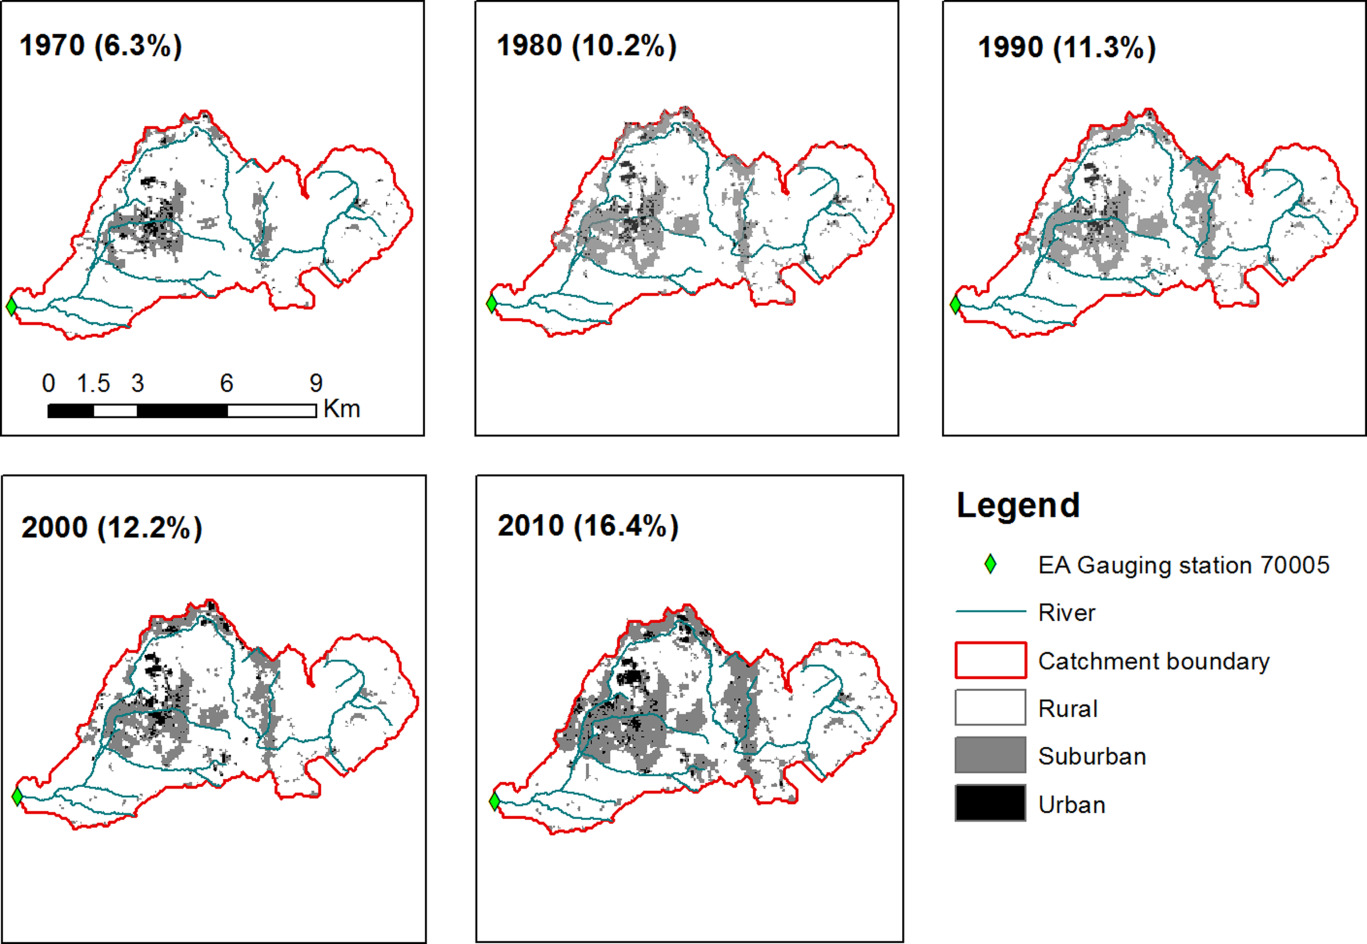
\includegraphics[width=0.87\textwidth]{wrcr21514-fig-0002-m} \end{center}

\footnotesize   from Prosdocimi et al.~(2015), WRR,
\url{doi:10.1002/2015WR017065}

\end{frame}

\begin{frame}{What causes change}
\protect\hypertarget{what-causes-change-1}{}

\begin{center}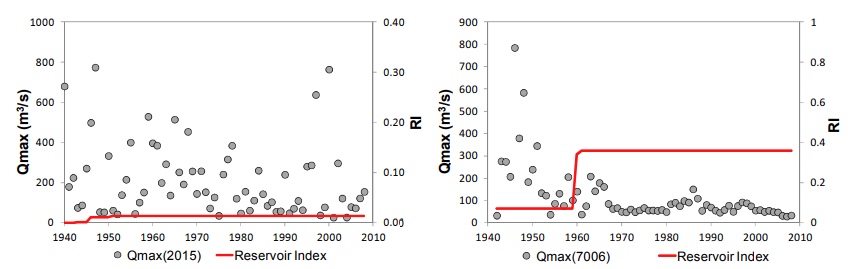
\includegraphics[width=0.98\textwidth]{ResIndex} \end{center}

~

\footnotesize   from Lopez Frances (2013), HESS,
\url{doi:10.5194/hess-17-3189-2013}

\end{frame}

\begin{frame}{What causes change}
\protect\hypertarget{what-causes-change-2}{}

\emph{Implicit} assumption:

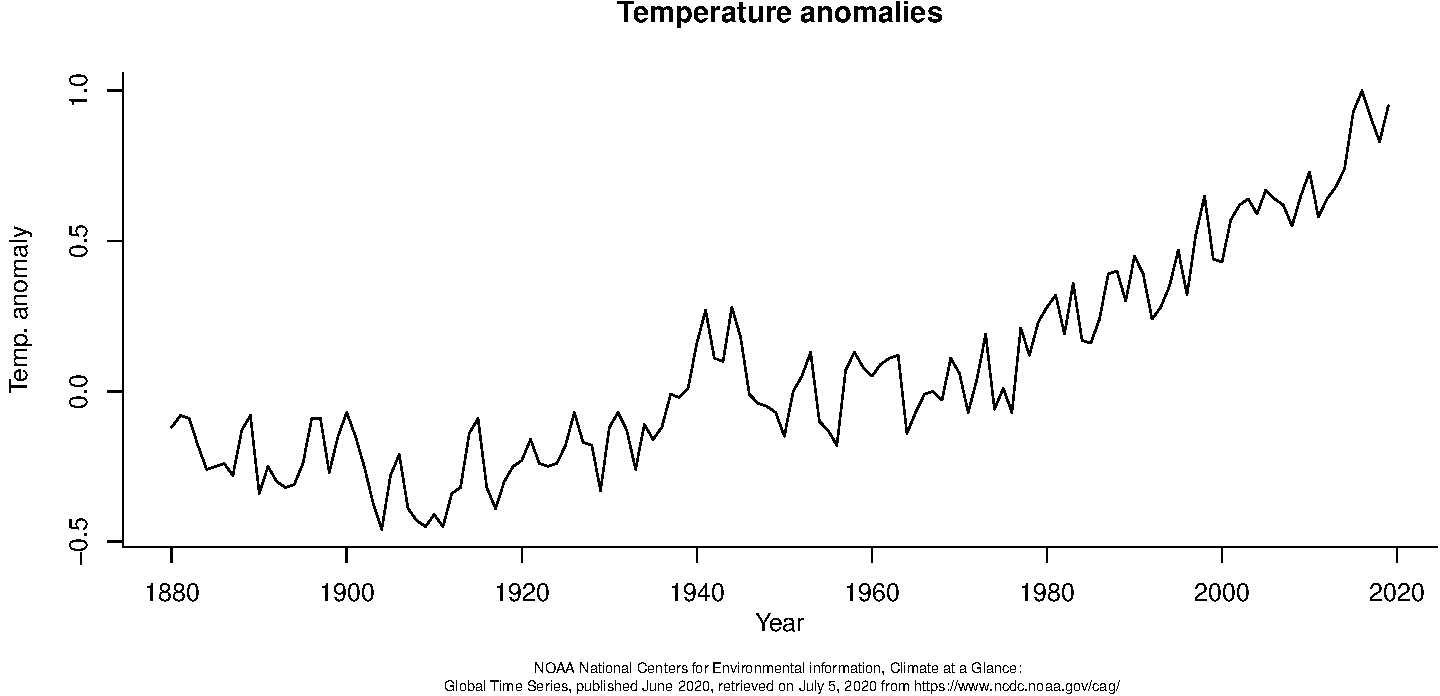
\includegraphics{ProsdocimiPerugia_files/figure-beamer/unnamed-chunk-1-1.pdf}

\end{frame}

\begin{frame}{Why study change?}
\protect\hypertarget{why-study-change}{}

\begin{itemize}
\tightlist
\item
  Understand if process of interest (river flow, rainfall, etc) is
  evolving in time
\item
  Understand how process of interest is affected by external drivers
\item
  Assess risk connected to a certain hazard and its evolution
\item
  If this is changing, how to account for this
\end{itemize}

~

Detection, \pause attribution \pause and management.

\end{frame}

\begin{frame}{The Lostock at Littlewood Bridge}
\protect\hypertarget{the-lostock-at-littlewood-bridge}{}

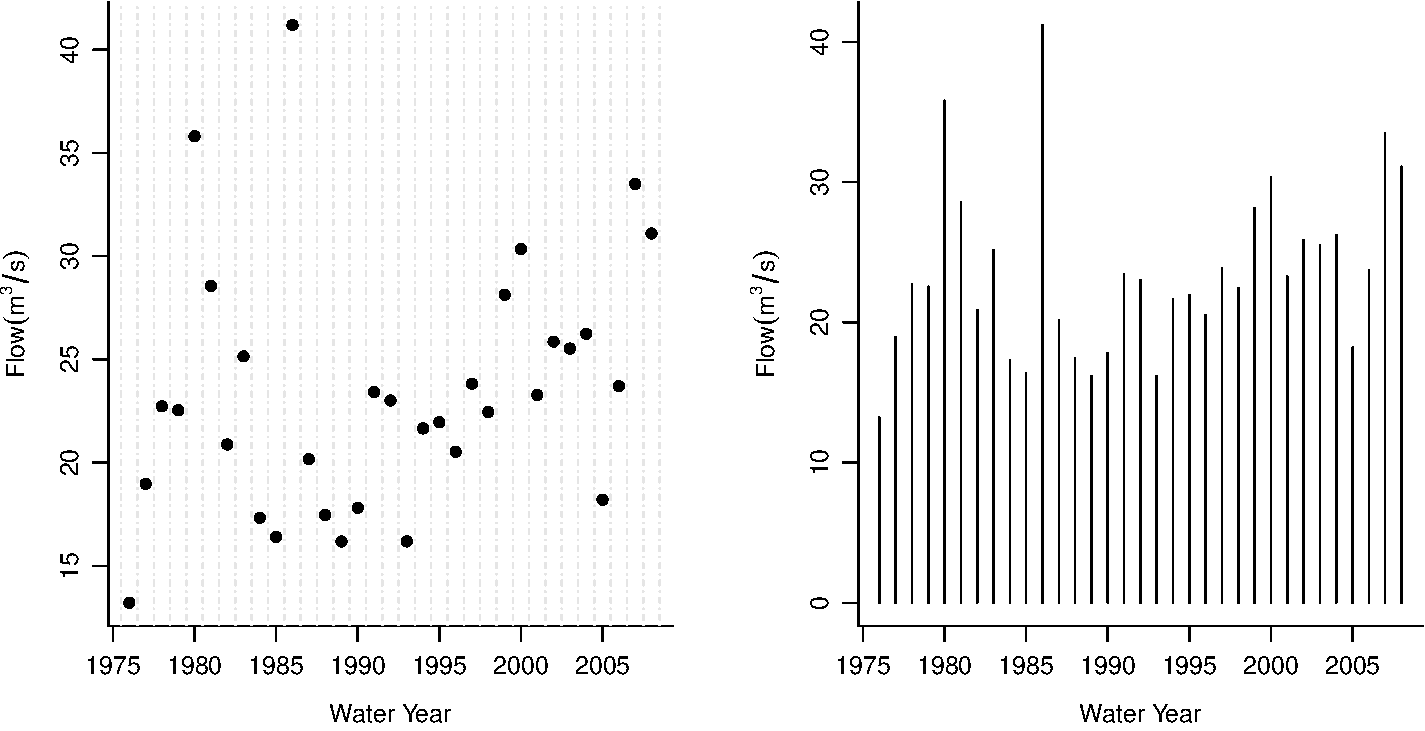
\includegraphics{ProsdocimiPerugia_files/figure-beamer/LostockData-1.pdf}

\end{frame}

\begin{frame}{The Lostock at Littlewood Bridge}
\protect\hypertarget{the-lostock-at-littlewood-bridge-1}{}

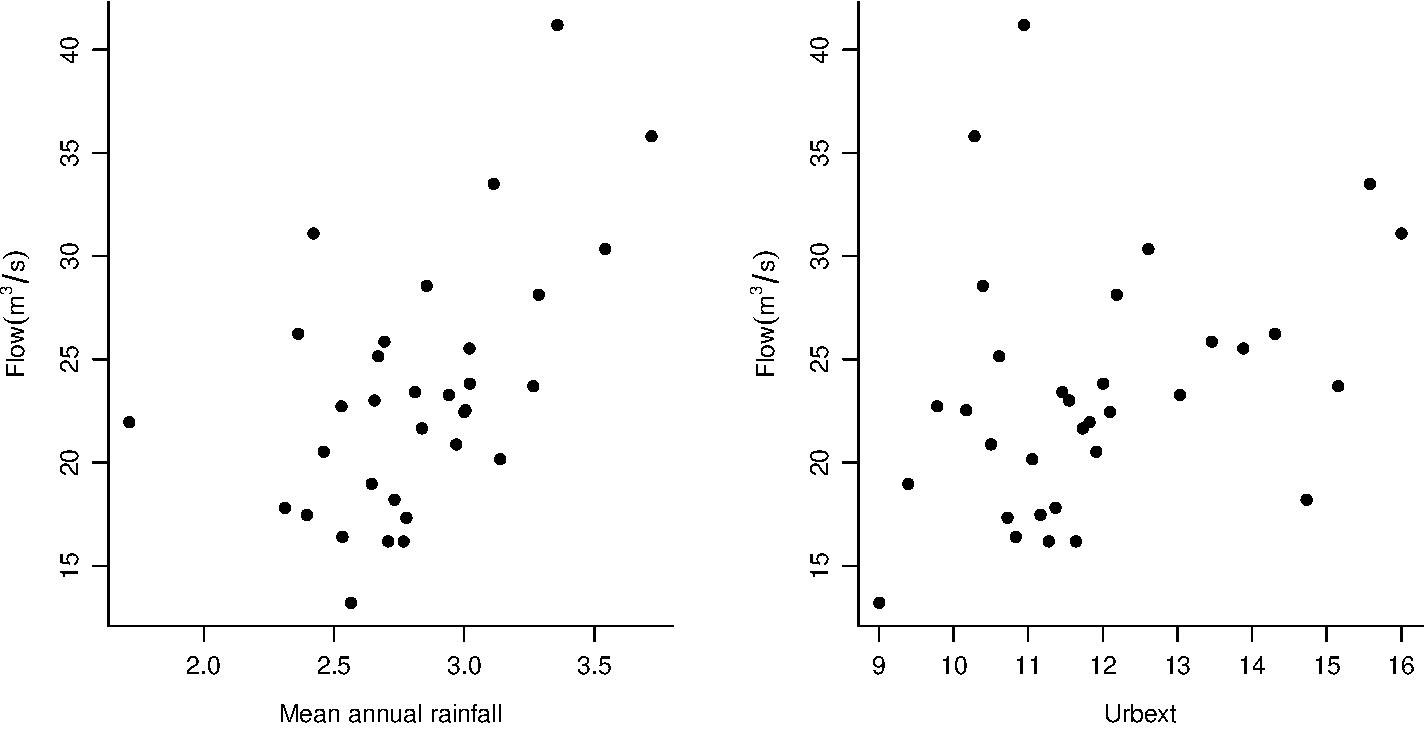
\includegraphics{ProsdocimiPerugia_files/figure-beamer/LostockDataExpl-1.pdf}

\end{frame}

\begin{frame}{Statistical tools}
\protect\hypertarget{statistical-tools}{}

We assume that \(\boldsymbol{y} = (y_1, \ldots, y_n)\) is a random
sample from a population.

We are interested in discovering some property of the population.

\pause

~

Inference framework:

\begin{itemize}
\tightlist
\item
  Parametric: assume that \(y_i\) is a realisation of some distribution
  described by \textbf{parameters} \(\boldsymbol{\theta}\)
  (\(f(y_i; \boldsymbol{\theta})\))
\item
  Non-parametric: no assumption on the distribution of \(f(y)\) is made
  (well, less assumptions\ldots)
\end{itemize}

\end{frame}

\begin{frame}{Parameteric framework}
\protect\hypertarget{parameteric-framework}{}

\linespread{1.5}

Advantage of parametric framework:

\begin{itemize}
\tightlist
\item
  Describe the whole distribution (including, for example, quantiles)
\item
  A very general framework
\item
  Easy to extend to very complex models (but estimation can be
  complicated)
\end{itemize}

~

\pause

The parametric framework:

\begin{itemize}
\tightlist
\item
  Assume that each member of the sample \(y_i\) comes from some
  distribution \(Y_i\)
\item
  Often assumed: \((Y_1, \ldots, Y_n)\) are independent and identically
  distributed (iid)
\item
  Assume that \(Y_i\) follows a known distribution parametrised by
  \(\boldsymbol{\theta}\)
\item
  (for example \(Y_i \sim N(\mu, \sigma)\), with
  \(\boldsymbol{\theta} = (\mu, \sigma)\))
\item
  Find estimates \(\hat{\boldsymbol{\theta}}\) based on the sample
\end{itemize}

\end{frame}

\begin{frame}{Estimation methods}
\protect\hypertarget{estimation-methods}{}

\begin{itemize}
\tightlist
\item
  Method of moments
\item
  Maximum likelihood
\item
  Bayesian approaches
\end{itemize}

\pause

Choice of framework and estimation method should depend on:

\begin{itemize}
\tightlist
\item
  Actual data properties
\item
  Main inferential question (and importance of uncertainty assessment)
\item
  Computational hurdle
\item
  Model complexity
\item
  Presence of prior information (which can be formalised)
\end{itemize}

\end{frame}

\begin{frame}{Maximum likelhood estimation}
\protect\hypertarget{maximum-likelhood-estimation}{}

The likelihood function is defined as
\[L(\boldsymbol{\theta}; \boldsymbol{y}) = \prod_{i=1}^{n} f(y_i, \boldsymbol{\theta}), \]
but calculations typically employ the log-likelihood
\[l(\boldsymbol{\theta}; \boldsymbol{y}) = \sum_{i=1}^{n} \log f(y_i, \boldsymbol{\theta}).\]
\(\hat{\boldsymbol{\theta}}_{ML}\) is the value that maximises
\(l(\boldsymbol{\theta}; \boldsymbol{y})\). \pause 

Asymptotically (\(n \rightarrow \infty\)) we have that
\(\hat{\boldsymbol{\theta}}_{ML} \sim N(\boldsymbol{\theta}, I_E(\boldsymbol{\theta})^{-1})\)
where \(I_E(\boldsymbol{\theta})\) is the expected information matrix,
with elements
\[e_{i,j}(\theta) = E\left[ - \frac{d^2 l(\theta)}{d \theta_i d \theta_j} \right] \]
Typically \(I_E(\boldsymbol{\theta})\) is unknown: use the observed
information matrix evaluated at \(\hat{\boldsymbol{\theta}}\).

\end{frame}

\begin{frame}{Parametric models for change}
\protect\hypertarget{parametric-models-for-change}{}

\begin{itemize}
\tightlist
\item
  Assume \(Y_i\) comes from a distribution
  \(f(\boldsymbol{\theta}_i,y_i)\)
\item
  Assume \(\boldsymbol{\theta}_i = g(\boldsymbol{x}_i)\)
\item
  So \(Y_i = (Y|X=x_i)\) with \(f(g(\boldsymbol{x}_i),y_i)\)
\end{itemize}

~

Example. Linear regression (with two explanatory variables):

\begin{itemize}
\tightlist
\item
  \(Y_i \sim N(\mu_i, \sigma)\);
  \(\boldsymbol{\theta}_i = (\mu_i, \sigma)\).
\item
  \(\mu_i = \beta _0 + \beta_1 x_{1i} + \beta_2 x_{2i}\) - linear
  relationship.
\item
  \(\sigma\) is constant.
\item
  As a consequence:
  \(E[Y_i] = \beta _0 + \beta_1 x_{1i} + \beta_2 x_{2i}\),
  \(V[Y_i] = \sigma^2\).
\item
  We can describe \(Y\) and how it varies with X
\end{itemize}

\end{frame}

\begin{frame}{Parametric models for change}
\protect\hypertarget{parametric-models-for-change-1}{}

Linear regression likelihood:

\[l(\boldsymbol{\theta}; \boldsymbol{y}) = \sum_{i=1}^{n} \log f(y_i, \boldsymbol{\theta}) \propto - n \log \sigma - \frac{(y-\beta _0 - \beta_1 x_{1i} - \beta_2 x_{2i})^2}{2 \sigma^2} \]
ML estimates can be derived analytically:
\((\hat{\beta}_0, \hat{\beta}_1,\hat{\beta}_2,\hat{\sigma})\).

And we have, for example,
\(\hat{\beta}_i \sim N(\beta_i, \hat{\sigma}_{\beta_i})\).

\pause

From this once can construct confidence intervals for \(\beta_i\) or
perform a test such as:
\[H_0: \beta_0 \geq \tilde{\beta} \quad \quad VS  \quad \quad H_1: \beta_0 < \tilde{\beta}\]
By default \(\tilde{\beta} = 0\), but one can test for any value
\(\tilde{\beta}\) and statistical test (\(=\), \(\leq\),
\(\geq\)).\footnote{Prosdocimi et al, NHESS, doi:10.5194/nhess-14-1125-2014}

Notice that if \(x_j\) is a factor one can account for step changes
(change points).

\end{frame}

\begin{frame}{Parametric models of change in extremes}
\protect\hypertarget{parametric-models-of-change-in-extremes}{}

Describing extremes is a different task than describing the typical
behaviour.

\((y_1, \ldots, y_n)\) is a sample of extremes: what is a reasonable
assumption for Y?

Extreme Value Theory gives theoretical derivation, but practice is often
different.

Regardless of the choice of \(f(y, \boldsymbol{\theta})\) - parametric
models of change for extremes can be easily constructed assuming
\(Y_i=(Y|X=x_i)\) and \(\boldsymbol{\theta}_i = g(\boldsymbol{x}_i)\).

\pause

What is an extreme?

\begin{itemize}
\tightlist
\item
  Largest event over a certain amount of time (eg water year, season)
\item
  Events larger than a certain high threshold (independent events?)
\end{itemize}

\end{frame}

\begin{frame}{Parametric models in extremes}
\protect\hypertarget{parametric-models-in-extremes}{}

Traditional (asymptotic) results based on extremes of stationary series:

\begin{itemize}
\tightlist
\item
  Block maxima: \(Y \sim GEV(\mu, \sigma, \xi)\)
\item
  Threshold exceedance magnitude: \(Y \sim GP(\sigma, \xi)\)
\item
  Threshold exceedance frequency: \(N \sim Pois(\lambda)\)
\end{itemize}

\pause  Using exceedances typically results in larger samples (so less
variability in estimates).

\pause

In practice other distributions are often assumed for Flow maxima.

\end{frame}

\begin{frame}{Generalised Extreme Value distribution}
\protect\hypertarget{generalised-extreme-value-distribution}{}

\[ \text{The GEV CDF:} \quad F(y, \boldsymbol \theta) =  \exp\left\{ -\left( 1 + \xi \frac{y-\mu}{\sigma} \right) ^{-1/\xi} \right\}\]
\(\boldsymbol\theta = (\mu, \sigma, \xi)\):

\begin{itemize}
\tightlist
\item
  \(\mu \in \mathbb{R}\): location parameter
\item
  \(\sigma > 0\); scale parameter
\item
  \(\xi \in \mathbb{R}\): shape parameter.
\end{itemize}

\(Y \sim GEV(\mu, \sigma,\xi)\) is defined on
\({y: 1 + \xi (y - \mu)/\sigma > 0}\), this means:

\begin{itemize}
\tightlist
\item
  \(y \in \left[ \mu -\sigma/\xi, \infty \right)\), if \(\xi > 0\)
  (Frechet)
\item
  \(y \in \left( -\infty, \mu -\sigma/\xi \right]\), if \(\xi < 0\)
  (Weibull)
\item
  \(y \in \left( -\infty, \infty \right)\), if \(\xi = 0\) (Gumbel)
\end{itemize}

BUT! In engineering/hydrology \(Y \sim GEV(\xi, \alpha, \kappa)\) and
\(\kappa = -\xi\). Software can use different parametrisation.

\end{frame}

\begin{frame}{Generalised Extreme Value distribution}
\protect\hypertarget{generalised-extreme-value-distribution-1}{}

\[\text{Quantile function (for $\xi \neq 0$)}: \ q(y, \theta) = \mu + \frac{\sigma}{\xi} \left[(-\log(1-p))^{-\xi} -1 \right] \]

\pause

Modelling change: \[ \mu = \mu_0+\mu_1 x\] \pause  Effective quantile
for \(x=x^*\):
\[\ q(y, \theta(x^*)) = \mu_0+\mu_1 x^* + \frac{\sigma}{\xi} \left[(-\log(1-p))^{-\xi} -1 \right] \]

\end{frame}

\begin{frame}{Changes in annual maxima - choice of distribution}
\protect\hypertarget{changes-in-annual-maxima---choice-of-distribution}{}

The Lostock at Littlewood Bridge: median and effective 50-yrs event.

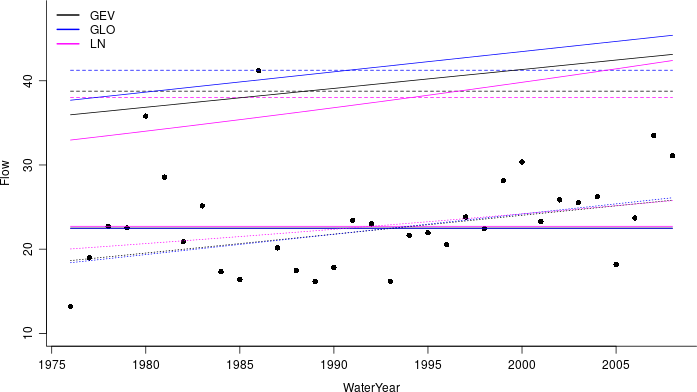
\includegraphics{ProsdocimiPerugia_files/figure-beamer/allRetsPlots-1.png}

\end{frame}

\begin{frame}{Changes in annual maxima}
\protect\hypertarget{changes-in-annual-maxima}{}

Time is not a cause for change, but land cover changes impact peak
flow.\\
\[\mu=\mu_0 + \mu_{urb} urb \quad \text{while } (\sigma, \xi)  \text{ constant }\]
\vspace{-1.2cm}

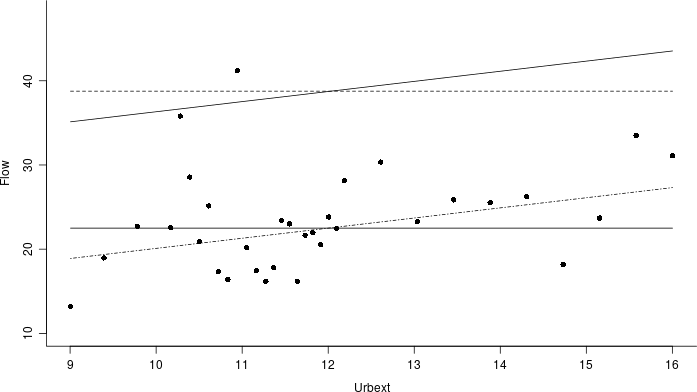
\includegraphics{ProsdocimiPerugia_files/figure-beamer/urbextRetPlot-1.png}

\end{frame}

\begin{frame}{Changes in annual maxima}
\protect\hypertarget{changes-in-annual-maxima-1}{}

Time is not a cause for change, but soil wetness impact peak flow.\\
\[\mu=\mu_0 + \mu_{rain} rain \quad \text{while } (\sigma, \xi)  \text{ constant }\]

\vspace{-1.0cm}

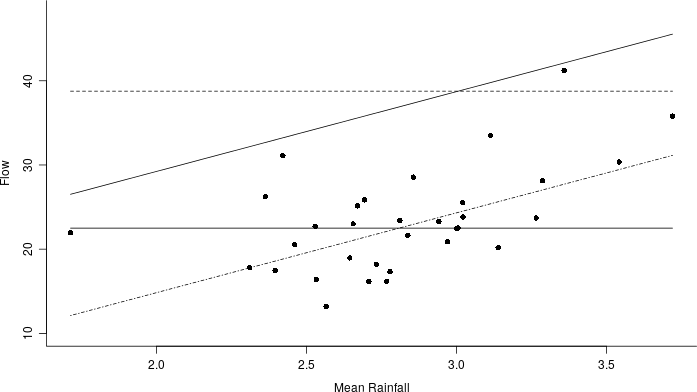
\includegraphics{ProsdocimiPerugia_files/figure-beamer/rainRetPlot-1.png}

\end{frame}

\begin{frame}{Changes in amax - effect of rain given Urbext}
\protect\hypertarget{changes-in-amax---effect-of-rain-given-urbext}{}

Separate effect of rain and urbanisation:\\
\vspace{-0.4cm}
\[\mu=\mu_0 + \mu_{rain} rain + \mu_{urb} urb \quad \text{while } (\sigma, \xi)  \text{ constant }\]
\vspace{-1.0cm}

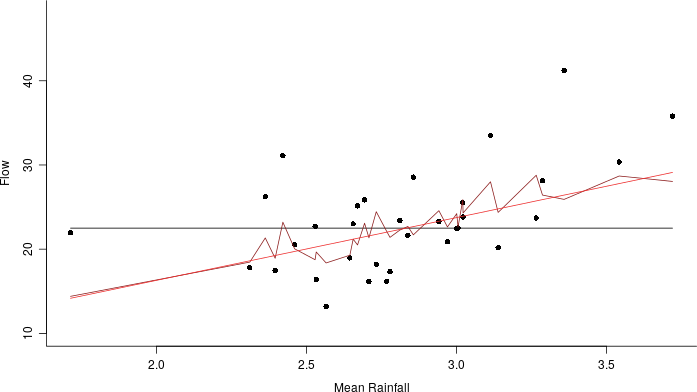
\includegraphics{ProsdocimiPerugia_files/figure-beamer/rainGivenUrbRetPlot-1.png}

\end{frame}

\begin{frame}{Changes in amax - effect of Urbext given rain}
\protect\hypertarget{changes-in-amax---effect-of-urbext-given-rain}{}

Separate effect of rain and urbanisation:\\
\vspace{-0.4cm}
\[\mu=\mu_0 + \mu_{rain} rain + \mu_{urb} urb \quad \text{while } (\sigma, \xi)  \text{ constant }\]
\vspace{-1.0cm}
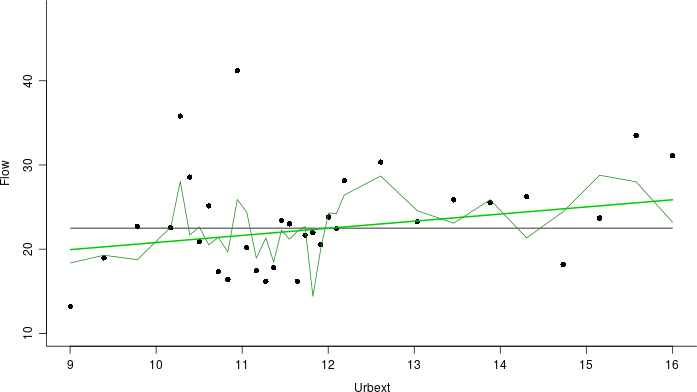
\includegraphics{ProsdocimiPerugia_files/figure-beamer/urbGivenRainRetPlot-1.png}

\end{frame}

\begin{frame}{Changes in annual maxima - estimated parameters}
\protect\hypertarget{changes-in-annual-maxima---estimated-parameters}{}

\linespread{1.0}\selectfont

Rain as covariate (log-lik: -98.39)

\begin{longtable}[]{@{}llllll@{}}
\toprule
& \(\mu_0\) & \(\mu_{urb}\) & \(\mu_{rain}\) & \(\sigma\) &
\(\xi\)\tabularnewline
\midrule
\endhead
MLE & -5.604 & - & 9.479 & 4.042 & 0.003\tabularnewline
se & 8.158 & - & 2.830 & 0.622 & 0.168\tabularnewline
\bottomrule
\end{longtable}

Urbext as covariate (log-lik: -100.0004)

\begin{longtable}[]{@{}llllll@{}}
\toprule
& \(\mu_0\) & \(\mu_{urb}\) & \(\mu_{rain}\) & \(\sigma\) &
\(\xi\)\tabularnewline
\midrule
\endhead
MLE & 6.53 & 1.20 & - & 4.17 & 0.04\tabularnewline
se & 4.79 & 0.40 & - & 0.60 & 0.13\tabularnewline
\bottomrule
\end{longtable}

Rain and urbext as covariate (log-lik: -96.47)

\begin{longtable}[]{@{}llllll@{}}
\toprule
& \(\mu_0\) & \(\mu_{urb}\) & \(\mu_{rain}\) & \(\sigma\) &
\(\xi\)\tabularnewline
\midrule
\endhead
MLE & -9.767 & 0.845 & 7.449 & 3.862 & -0.016\tabularnewline
se & 7.344 & 0.422 & 2.668 & 0.580 & 0.153\tabularnewline
\bottomrule
\end{longtable}

\end{frame}

\begin{frame}{Changes in extremes - attribution}
\protect\hypertarget{changes-in-extremes---attribution}{}

Kendall's \(\hat{\tau}\)(Urbext, Rain) = 0.068.

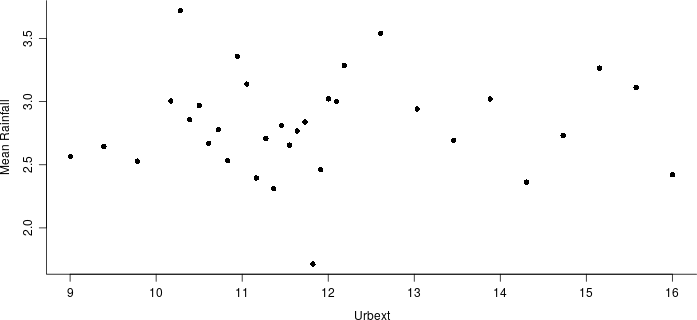
\includegraphics{ProsdocimiPerugia_files/figure-beamer/urbAndRain-1.png}

\pause

Reality is complex: linear models are a (over-simplified!)
representation.

\end{frame}

\begin{frame}{Changes is peaks over threshold}
\protect\hypertarget{changes-is-peaks-over-threshold}{}

Extract observations above a high threshold

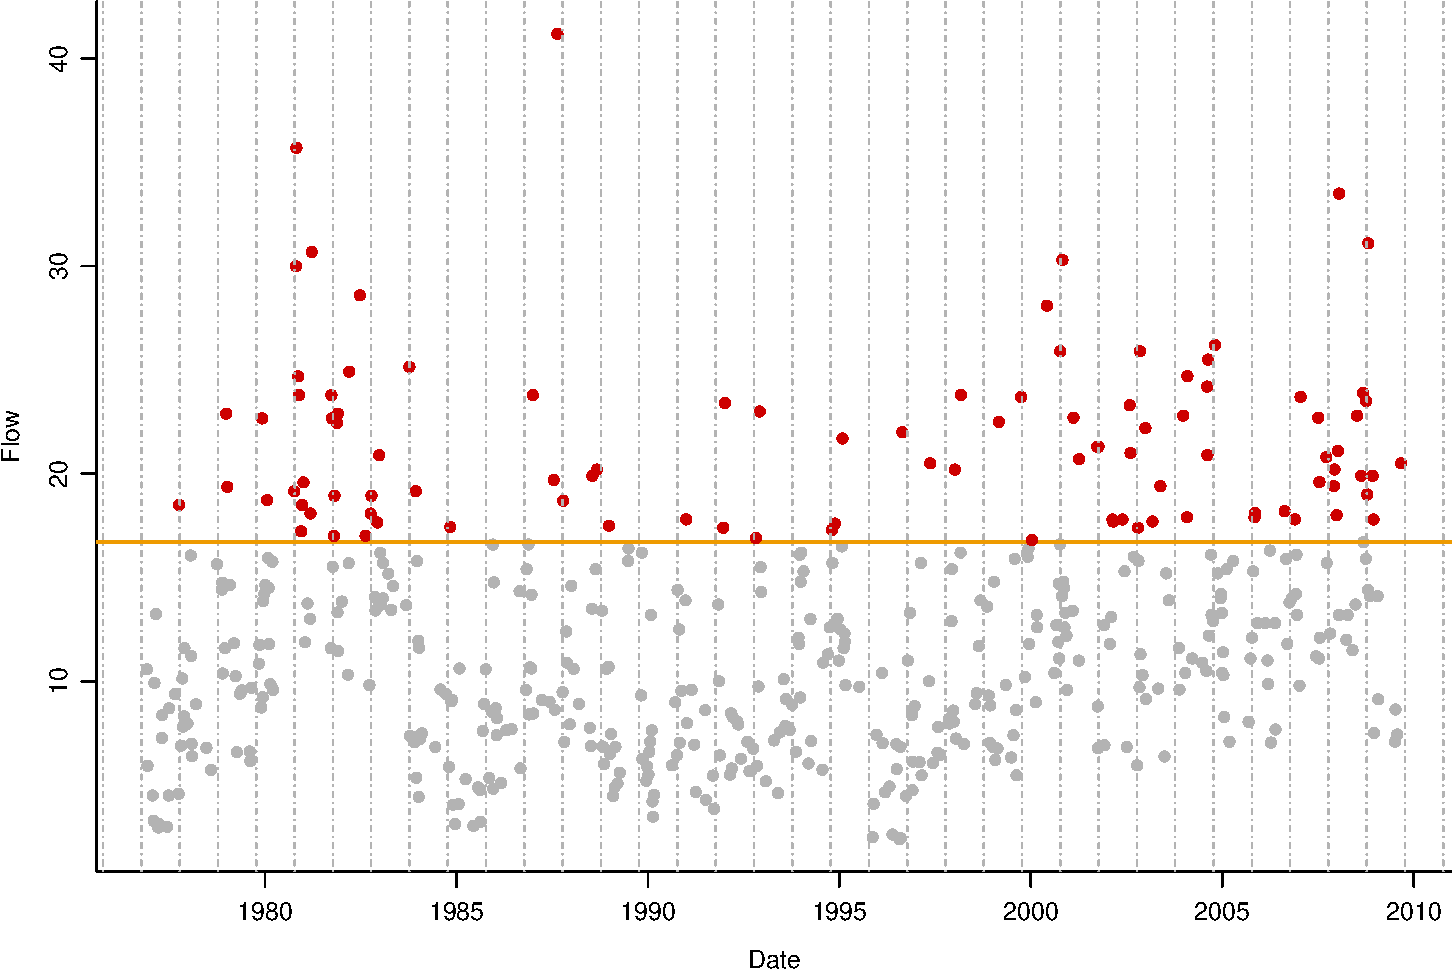
\includegraphics{ProsdocimiPerugia_files/figure-beamer/unnamed-chunk-5-1.pdf}

\end{frame}

\begin{frame}{Generalised Pareto Distribution}
\protect\hypertarget{generalised-pareto-distribution}{}

\(Y\) is taken to be the observations above a high threshold \(u\)
(\(Y = (X|X>u)\)).

GP is the limiting distribution for the magnitude of exceedances.
\[F(y, u, \boldsymbol \theta) =  1- \left( 1 + \xi \frac{y-u}{\tilde{\sigma}} \right) ^{-1/\xi}\]
\(u\) is a constant, \(\boldsymbol\theta = (\sigma, \xi)\):

\begin{itemize}
\tightlist
\item
  \(\sigma > 0\); scale parameter
\item
  \(\xi \in \mathbb{R}\): shape parameter.
\end{itemize}

The domain changes depending on the sign of \(\xi\):
\(y \in \left[u, \infty \right)\), if \(\xi \geq 0\);
\(y \in \left( -\infty, u -\sigma/\xi \right]\), if \(\xi < 0\).

\[ \text{Quantile function:}\quad  q(p, u, \boldsymbol \theta) = u + \frac{\sigma}{\xi} (p^{-\xi} - 1) \]

\pause

Modelling change: \(\sigma_0 + \sigma_1 x\)

\end{frame}

\begin{frame}{Point Process representation of extremes}
\protect\hypertarget{point-process-representation-of-extremes}{}

Exceedances frequency and magnitude traditionally modelled as separate
processes.

They can be modelled in a unique framework using a Point Process
representation of extremes
\footnote{Smith, Statist. Sci., doi:10.1214/ss/1177012400}. \pause This
representation is under-utilised in hydrology.

\(N\) = \{no. Exceedance in a Year\}. \(N \sim Pois(\lambda)\)

\(P(\text{no. Exceedance in a Year})\) is linked to magnitudes.

\pause

Express this using GEV-parameters:

\[\log \lambda = -\frac{1}{\xi} \log\left[1+\xi \frac{u-\mu}{\sigma} \right]\]

\pause

Express changes in magnitude and frequency in the same model

Same meaning as GEV models of change

\end{frame}

\begin{frame}{Changes in Peaks - Point Process}
\protect\hypertarget{changes-in-peaks---point-process}{}

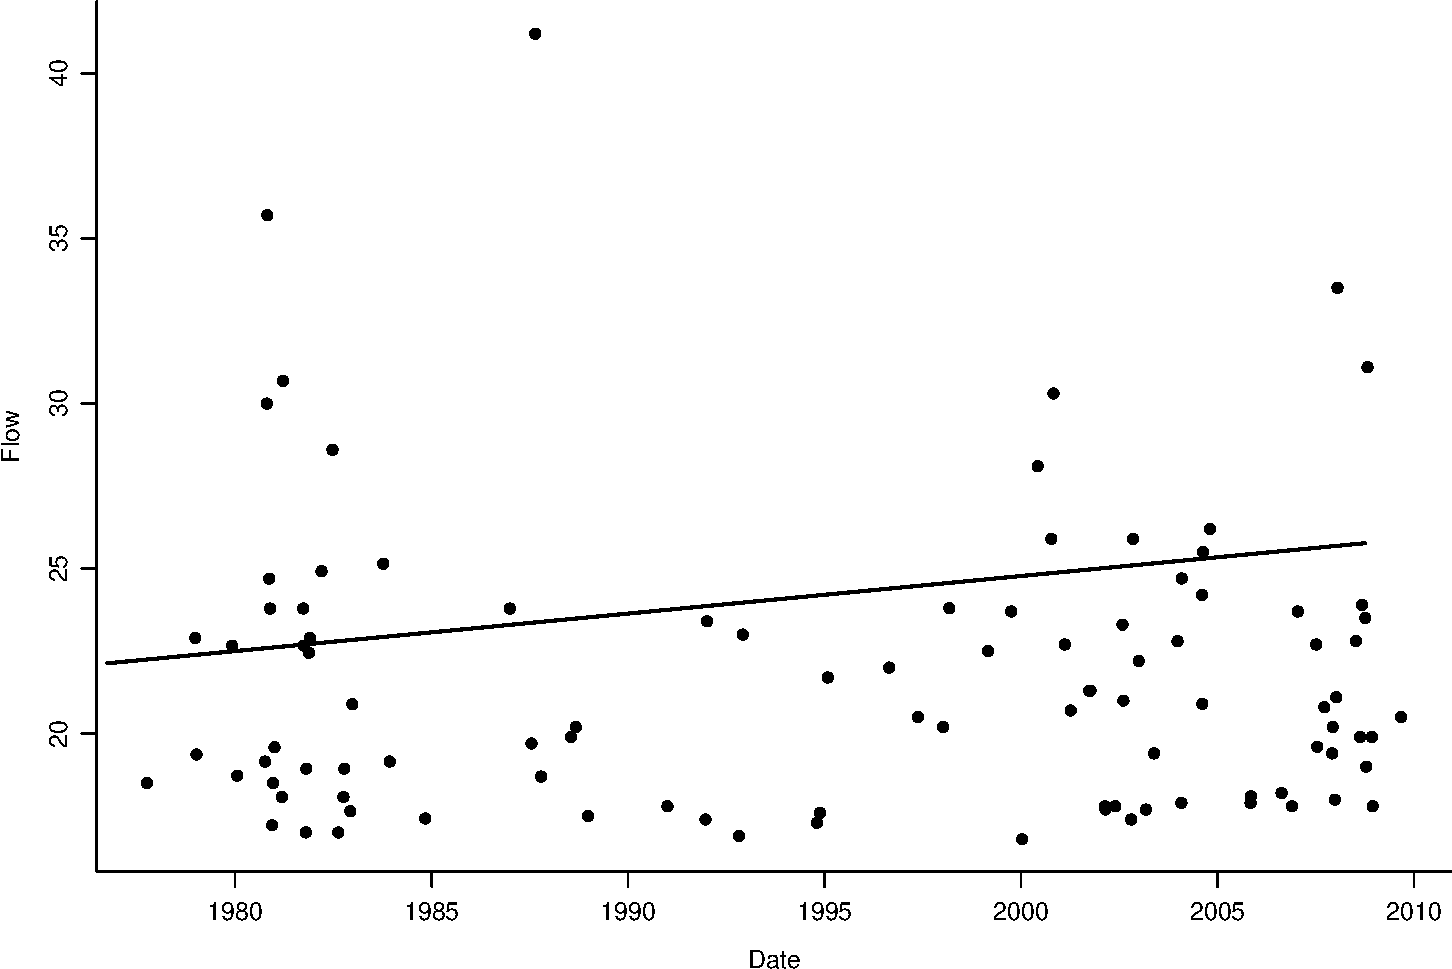
\includegraphics{ProsdocimiPerugia_files/figure-beamer/ppFirstPlot-1.pdf}

\end{frame}

\begin{frame}{Changes in extremes - comparing the models}
\protect\hypertarget{changes-in-extremes---comparing-the-models}{}

Rain and urbext as covariate - GEV:

\begin{longtable}[]{@{}llllll@{}}
\toprule
& \(\mu_0\) & \(\mu_{urb}\) & \(\mu_{rain}\) & \(\sigma\) &
\(\xi\)\tabularnewline
\midrule
\endhead
MLE & -9.767 & 0.845 & 7.449 & 3.862 & -0.016\tabularnewline
se & 7.344 & 0.422 & 2.668 & 0.580 & 0.153\tabularnewline
\bottomrule
\end{longtable}

\vspace{-0.2cm}

Rain and urbext as covariate - PP:

\begin{longtable}[]{@{}llllll@{}}
\toprule
& \(\mu_0\) & \(\mu_{urb}\) & \(\mu_{rain}\) & \(\sigma\) &
\(\xi\)\tabularnewline
\midrule
\endhead
MLE & -12.139 & 0.930 & 8.007 & 4.622 & -0.184\tabularnewline
se & 6.757 & 0.320 & 1.723 & 0.368 & 0.064\tabularnewline
\bottomrule
\end{longtable}

\pause

Larger sample size leads to more precise estimation (statistically)

Tail estimate is quite different

\end{frame}

\begin{frame}{Changes in extremes}
\protect\hypertarget{changes-in-extremes}{}

Parametric approaches: easy to include predictors and test for
significance

\pause

This might be a bug and not a feature

\pause

The assumption is that \(Y_i=(Y|X = x_i)\) follows
\(f(y; \boldsymbol \theta)\) - goodness of fit should be carried out on
\textbf{residuals}

Statistical EVT and practice are not aligned

\end{frame}

\begin{frame}{Detection}
\protect\hypertarget{detection}{}

Methods sometimes chosen because of data availability

Statistical models rely on assumption of iid random observations

Short records: hard to identify complex evolutions

Short records: hard to observe a good range of the explantory variable

When detecting ``change'': what are we
detecting?\footnote{Merz et al, HESS, doi:10.5194/hess-16-1379-2012}

\end{frame}

\begin{frame}{Attribution}
\protect\hypertarget{attribution}{}

Golden standard of causality is randomised trials: what about
observational studies?

Climate sciences reproduce the treatment/placebo framework with
numerical experiments (how good for extremes?).

Some numerical experiments done in hydrology - but systems are complex.

Causality: a cascade of impacts (with
feedback\footnote{Zhang et al, Nature, doi:10.1038/s41586-018-0676-z})

\end{frame}

\begin{frame}{Changes in annual maxima - uncertainity}
\protect\hypertarget{changes-in-annual-maxima---uncertainity}{}

Structures are designed for the ``T-Year'' event: estimated as the 1-1/T
quantile.

If the distribution is changing so is the quantile.

\pause

\begin{longtable}[]{@{}lrrrr@{}}
\toprule
& Q100 & 95\% lb & 95\% ub & width\tabularnewline
\midrule
\endhead
no-change & 30.514 & 41.837 & 53.159 & 11.322\tabularnewline
Rain = max(Rain) & 33.676 & 48.403 & 63.130 & 14.727\tabularnewline
\bottomrule
\end{longtable}

Adding parameters adds variation to the estimates - is it worth it?

\pause

Bias-variance trade-off and parsimonious models.

\end{frame}

\begin{frame}{Changes in extremes - consequences}
\protect\hypertarget{changes-in-extremes---consequences}{}

How to quantify risk under
change?\footnote{Volpi, Wires Water, doi:10.1002/wat2.1340}

Choice of distribution has an impact on estimates of rare events

Today I used ``effective design events'':
\(q(p; \hat{\boldsymbol \theta})\). So at \(X=x^{*}\):
\(q(p; \hat{\boldsymbol \theta}(x^{*}))\).

Choice of distribution/model has an impact on estimates of rare events.

Choice of model has an impact of description of
change\footnote{Vogel et al JAWRA doi:10.1111/j.1752-1688.2011.00541.x}.
\[\text{GEV quantile function (for $\xi \neq 0$)}: \ q(y, \theta) = \mu + \frac{\sigma}{\xi} \left[(-\log(1-p))^{-\xi} -1 \right] \]

Compare effective return levels for \(x^{*}\) and \(x_0\):
\[q(p; \hat{\boldsymbol \theta}(x^{*})) - q(p; \hat{\boldsymbol \theta}(x_0)) = \mu_1 (x^{*}-x_0)\]

\end{frame}

\begin{frame}{(Statistical) recommended reading}
\protect\hypertarget{statistical-recommended-reading}{}

Coles, S (2001), An introduction to statistical modeling of extreme
values, Springer

Katz, R.W., Parlange, M.B. and Naveau, P., 2002. Statistics of extremes
in hydrology. Advances in water resources, 25(8-12), pp.1287-1304.

Katz, Richard (2013) Statistical Methods for Nonstationary Extremes,
Chapter 2 in A. AghaKouchak et al.~(eds.), Extremes in a Changing
Climate, Water Science and Technology Library 65, DOI
10.1007/978-94-007-4479-0 2,

\end{frame}

\begin{frame}{Doing science the right way}
\protect\hypertarget{doing-science-the-right-way}{}

Reproducibility crisis in several fields - open science movement as a
result.

Replicability (i.e.~being able to re-run the analysis) should be a
given.

Start any project in a replicable way: literate programming and
programmatic interaction with data (access, manipulation, analysis).

In R (and Python) this is increasingly feasible.

Slides code at
\href{https://github.com/ilapros/PerugiaSummerSchool/tree/master/July2020}{github.com/ilapros}

\end{frame}

\end{document}
